\documentclass[11pt]{article}
\usepackage[spanish]{babel}
\usepackage[utf8]{inputenc}
\usepackage[T1]{fontenc}
\usepackage{graphicx}
\topmargin=-1.2cm
\textheight=22cm
\textwidth=16cm  
\oddsidemargin=0.45cm  
\setlength{\parindent}{0cm}
\renewcommand{\baselinestretch}{1.1}
\graphicspath{{hola/}}
\title{Actividad 5}
\author{Hinostroza Moya Natalia}
\date{08 de marzo de 2017}

\begin{document}
%===============================================================================
% PORTADA
%===============================================================================
\begin{titlepage}
\begin{center}
\includegraphics[scale=0.35]{escudo.png}
\end{center}
\vspace*{0.02in}
\begin{center}

\rmfamily\textbf{\LARGE UNIVERSIDAD DE SONORA}\\
\vspace*{1.02in}
{\Large División de Ciencias Exactas y Naturales}\\
{\Large Departamento de Física}\\

\vspace*{0.99in}
\rule{99mm}{0.1mm}\\
\vspace*{0.4cm}
\textbf{\LARGE Mareas y Corrientes}\\
\vspace*{0.001in}
\rule{99mm}{0.1mm}

\vspace*{1in}
\normalsize{Autor:}\
\normalsize{Natalia Hinostroza Moya}\\
\vspace*{0.3mm}
\normalsize Profesor:\
\normalsize Carlos Lizárraga Celaya\\
\vspace*{1.5cm}
\normalsize 14 de marzo de 2017

\end{center}
\end{titlepage}

%==============================================================================
% DESARROLLO
%==============================================================================
%%%Encabezamiento y pie de página

\textbf{\section*{\LARGE Resumen}}
En el suguiente reporte presentamos los resultado obtenidos para la actividad 5 de la clase de computacional. En esta se nos pide realizar una sintesis hacerca de las mareas. Tambien comenzaremos a trabajar con datos obtenidos en sondeos de mareas de distintas locaciones que presenta el Centro de Investigación Científica y de Educación Superior de Ensenada (CICESE), y el National Oceanic and Atmospheric Administration (NOAA). Los lugares de los que se obtuvieron los datos presentados en esta actividad son  de Mazatlán, Sinaloa, y de San Diego, California.\\

Los enlaces de las páginas web de las que se descargaron los datos aparecen al final de dicho reporte, en la bibliografía.

\textbf{\section{\LARGE Introducción}}
\large En actividades pasadas estudiamos los cambios atmósfericos y a qué se debían. Esta vez, de manera parecida a las actividades que ya hemos hecho anteriormente, estudiaremos a profundidad qué son las corrinetes marinas y las mareas. Para ello realizaremos la sintesis del artículo \underline{Mareas de la Wikipedia}.\\

El principal propósito de la siguiente sintesis es crearnos un mejor conocimiento hacer de que son las mareas, por que son provocadas, los estudios que se han realizado con ellas, entre otros aspectos importantes; ya que proximamente estaremos trabajando con sondeos de mareas de las regiones que elegidas.\\

Los cuadros que aparecen a final muestran los 10 principales componentes armónicos de la marea en los lugares que escogímos, junto a la descripción de su nombre, símbolo y periodo en horas.\\

\textbf{\section{\LARGE Mareas}}
\large Podemos definir a las mareas como los cambios en la najada y subida en el nivel del mar. Las mareas son causadas por los efectos combinados de distintas fuerzas gravitatorias ejercidas por la luna y el sol, así como por la rotación de la tierra. Las mareas pueden variar en escalas de tiempo que van desde horas a años por distintos factores. Dichos cambios son registrados con presición gracias a las estaciones medidoras de mareas que miden el nivel del agua a lo largo del tiempo.\\

Aunque la mareas suelen ser la principal razón de fluctuaciones a corto plazo del nivel del mar, los niveles del mar también pueden variar por otras fuerzas, como lo son el viento y cambios de la presión barométrica. Dichos fenómenos no sólo aparecen en los océanos, ocurren en cualquier otro sistema siempre que exista un campo gravitacional que varíe en tiempo y espacio. 

\begin{center}
\includegraphics[scale=0.60]{Imagen1.png}
\end{center}


\textbf{\section{\LARGE Características de las Mareas}}

Las etapas de los cambios de mareas son las siguientes:\\ 

\begin{enumerate}
\item El nivel del mar se eleva durante varias horas, cubriendo la zona intermareal; pleamar.
\item El agua sube a su nivel más alto, alcanzando la marea alta.
\item El nivel del mar cae durante varias horas, revelando la zona intermareal; reflujo.
\item El agua deja de caer, alcanzando la marea baja.
\end{enumerate}

Se conoce cómo corriente de marea a las corrientes oscilantes que son producidas por las mareas. Al momento en que estas corrientes cesan se le llama agua floja o marea floja, y suele producirse cerca de las aguas altas y bajas. Después, la marea invierte su dirección y se dice que está girando.\\

Muy comúnmente las mareas son semidiurnas, esto se refiere a que hay dos aguas altas o dos aguas bajas por día, o diurnas, un ciclo de marea por día.\\

\textbf{\subsection{\Large Definicion de las Mareas}}
Se presentan a continuación los tipos de mareas a partír del nivel más alto hasta el más bajo.\\

\begin{itemize}
\item\textbf{Highest Astronomical Tide (HAT):} La marea más alta que puede ser predecida. Hay que tener en cuenta que las condiciones meteorológicas pueden agregar altura adicional a este tipo de mareas.
\item\textbf{Mean High Water Springs (MHWS):} Es el promedio de dos mareas altas en los días de mareas de primavera
\item\textbf{Mean High Water Neaps (MHWN):} Es el promedio de las dos mareas altas en dias de marea muerta.
\item\textbf{Mean Sea Level (MSL):}Este es el nivel medio del mar. El MSL es constante para cualquier localización durante un período largo. 
\item\textbf{Mean Low Water Neaps (MLWN):} Es el promedio de las dos mareas bajas en tiempod de marea muerta.
\item\textbf{Mean Low Water Springs (MLWS):} El promedio de las dos mareas bajas en épocas de mareas de primavera.
\item\textbf{Lowest Astronomical Tide (LAT) y Chart Datum (CD):} Es la marea más baja que puede se predecida. Se debe de tener en cuenta que en ciertas condiciones meteorológicas se puede mostrar un nivel de agua más bajo del que es realmente. 
\end{itemize}

\hspace{0.0001mm}
\begin{center}
\includegraphics[scale=0.40]{Imagen2.png}
\end{center}

\textbf{\section{\LARGE Componentes de las Mareas}}
Los componentes primarios constituyentes de las mareas son la rotación de la Tierra, La posición de la luna y el solen relación con la Tierra, la elevación de la luna sobre el ecuador y la batimetría. La variaciones que tienen períodos menores de medio de día son llamadas constituyentes armónicas, y las que duran días, meses o años son reconocidas como constituyentes de largo período.\\

\textbf{\subsection{\Large Principales componentes semidiurnos lunares}}
El periodo de este es mas o menos de 12 horas y 25.2 minutos, exactamente la mitad de un día lunar de marea. La luna orbita alrededor dela Tierra en la misma dirección en que la Tierra rota en su eje, así que toma un poco más de un día,aproximadamente24 horas con 50 minutos, para Luna en regresar al mismo lugar en el cielo.\\ 

Ya que el campo gravitatorio creado por la luna se devilita con la distancia, ejerce una fuerza ligeramente más fuerte que la media del lado en que está frente a la Tierra y una ligeramente más débil en el lado opuesto. Así, la luna tiende a "estirar" ligeramente la Tierra a lo largo de la linea que une ambos cuerpos. La Tierra, al ser sólida, sólo se deforma un poco, pero el agua del océano, siendo un fluido, tiene la libertad de moverse mucho más en respuesta a la fuerza de marea, particularmente de forma horizontal. Aunque el océano nunca alcanza el equilibrio nunca hay tiempo para que el fluido alcance el estado al que eventualmente llegaría si la fuerza de marea fuera constante.\\

Cuando hay dos mareas altas cada día con difeentes alturas (y dos bajas, también con alturas distintas), el patrón se denomina marea semi-diurna mixta. 

\textbf{\subsection{\Large Variación de rango: springs y mareas muertas}}
El rango semi-diurno (diferencia de altura entre las aguas altas y bajas durante aproximadamente medio día) varía en un ciclo de dos semanas. Aproximadamente dos veces al mes, alrededor de la luna nueva y la luna llena, cuando el sol, la Luna y la Tierra están alineados (condición conocida como syzygy), la fuerza de marea se vuelve mayor. El margen de la marea está entonces está en su máximo. Esto es conocido como "the spring tide", no se nombran así por la estación, si no por que esta palabra deriva del signifaco "salto, estallido, subida", como un resorte natural.\\ 

Cuando la Luna y el Sol están separados por 90$^{\circ}$ al verse desde la Tierra, la fuerza de marea solar cancela parcialmente la lunar. En estos puntos del ciclo lunar, el margende las mareas está en su mínimo. Esto es conocido como la marea muerta. 

\textbf{\subsection{\Large Altitud lunar}}
La distancia cambiante entre la Luna y la Tierra también afecta las alturas de las mareas. Cuando la Luna está más cerca, en el perigeo, la gama aumenta, y cuando está en el apogeo, la gama se encoge.

\textbf{\subsection{\Large Otros factores}}
Se tiene el efecto gravitacional solar, la oblicuidad del ecuador de la Tierra y rotación de eje, la inclinación de la Tierra de la órbita lunar  y de la forma elíptica  de la órbita terrestre del sol.

\textbf{\subsection{\Large Fase y amplitud}}
La etapa o fase de una marea, denotada por el tiempo en horas después del alto nivel de agua, es un concepto útil. La etapa de marea también se mide en grados, con 360$^{\circ}$ por ciclo de marea. Las líneas de fase constante de marea se llaman líneas cotidal, que son análogas a líneas de contorno de altitud constante en mapas topográficos.\\

El agua alta gira alrededor del punto anfidrómico una vez cada 12 horas en la dirección de las líneas cotidalas ascendentes, y lejos de la disminución de las líneas cotidal. Esta rotación es generalmente en sentido horario en el hemisferio sur y en sentido contrario a las agujas del reloj en el hemisferio norte, y es causada por el efecto Coriolis. La diferencia de la fase cotidal de la fase de una marea de referencia es la época. La marea de referencia es el constituyente hipotético "marea de equilibrio" en una Tierra sin tierra medida a 0$^{\circ}$ de longitud, el meridiano de Greenwich.

\textbf{\section{\LARGE Física}}
\textbf{\subsection{\Large Historia de la física de mareas}}
El estudio de la física de mareas fue importante en el desarrollo temprano de heliocentrismo y la mecánica de los cuerpos celestes, con la existencia de dos mareas diarias explicadas por la gravedad de la Luna. Más tarde tambien se estudio el efecto del Sol en las mareas.\\

El primero en ingresar la teoría de que las mareas eran causadas por la luna fue Seleucus de Seleucia, alrededor del año 150 aC. Despues de él vinieron muchos más científicos cómo Kepler, Galileo Galilei, Newton, entre otros, que continuaron estudiando las fuerzas que actuan sobre la tierra y que repercuten en la producción de las mareas. 

\textbf{\subsection{\Large Fuerzas}}
La fuerza de marea producida por un objeto masivo (Luna, en adelante) sobre una pequeña partícula situada sobre o en un cuerpo extenso (Tierra, en adelante) es la diferencia vectorial entre la fuerza gravitacional ejercida por la Luna sobre la partícula y la fuerza gravitatoria que se ejercería sobre la partícula si estuviera situada en el centro de masa de la Tierra.\\

La fuerza gravitacional solar en la Tierra es en promedio 179 veces más fuerte que la lunar, pero debido a que el Sol está en promedio 389 veces más lejos de la Tierra, su gradiente de campo es más débil. La fuerza de marea solar es 46\% tan grande como el lunar.

\textbf{\subsection{\Large Ecuación de mareas de Laplace }}
Las profundidades oceánicas son mucho más pequeñas que su extensión horizontal. Por lo tanto, la respuesta al forzamiento de marea puede ser modelada utilizando las ecuaciones de marea de Laplace. Esta incorpora las siguientes característica:\\

\begin{enumerate}
\item La velocidad vertical (o radial) es despreciable.
\item  El forzamiento es sólo horizontal (tangencial).
\item El efecto de Coriolis aparece como una fuerza inercial (ficticia).
\item   La velocidad de cambio de la altura de la superficie es proporcional a la divergencia negativa de la velocidad multiplicada por la profundidad.
\end{enumerate}

\textbf{\subsection{\Large Amplitud y ciclos de tiempo }}

La amplitud teórica de las mareas oceánicas causada por la luna es de unos 54 centímetros (21 pulgadas) en el punto más alto, lo que corresponde a la amplitud que se alcanzaría si el océano poseía una profundidad uniforme, no había masas terrestres y la Tierra giraba en el paso con la órbita de la luna. El sol también causa mareas, de las cuales la amplitud teórica es de unos 25 centímetros (el 46\% de la de la luna) con un tiempo de ciclo de 12 horas. En la marea de primavera los dos efectos se suman unos a otros a un nivel teórico de 79 centímetros (31 pulgadas), mientras que en marea baja el nivel teórico se reduce a 29 centímetros (11 pulgadas).

\textbf{\subsection{\Large Disipación}}
Las oscilaciones de las mareas de la Tierra introducen la disipación a una velocidad promedio de unos 3.75 terawatts. Alrededor del 98\% de esta disipación es por mareas marinas. Estas se producen cuando los flujos de marea a escala de cuenca fluyen hacia los flujos de menor escala que experimentan una disipación turbulenta. 

\textbf{\subsection{\Large Batimetría}}
Las características costeras, como la batimetría submarina y la forma de la línea costera, hacen que las características de ubicación individual afecten el pronóstico de mareas; El tiempo y la altura reales del agua alta pueden diferir de las predicciones del modelo debido a los efectos de la morfología costera sobre el flujo de las mareas. Sin embargo, para un lugar dado, la relación entre la altitud lunar y el tiempo de marea alta o baja (el intervalo lunitidal) es relativamente constante y predecible, como es el tiempo de marea alta o baja con respecto a otros puntos de la misma costa.\\

Las masas terrestres y las cuencas oceánicas actúan como barreras contra el agua que se mueve libremente alrededor del globo, y sus formas y tamaños variados afectan el tamaño de las frecuencias de marea. Como resultado, los patrones de marea varían.\\

\textbf{\section{\LARGE Principales Componentes Armónicos de las Mareas}}
% TABLA 
\begin{table}[htbp]
\begin{center}
\begin{tabular}{|l|l|l|}
\hline \hline
Nombre & Símbolo & Periodo (hrs)  \\
\hline \hline
Límite de agua superficial de la luna principal & $M_{4}$ & 6.210300601 \\ \hline
Límite de agua superficial de la luna principal & $M_{6}$ & 4.140200401 	\\ \hline
Agua superficial terdiurnal & $MK_{3}$ & 8.177140247 \\ \hline
Abundancia de agua poco profunda de la energía solar principal & $S_{3}$ & 6 \\ \hline
Cuarto de agua poco profunda diurna &  $MN_{4}$  & 6.269173724 \\ \hline
Principal lunar semidiurno & $M_{2}$ & 12.4206012 \\ \hline
Principal solar semidiurno & $S_{2}$ & 12 \\ \hline
Gran lunar elíptica semidiurna & $N_{2}$ & 12.65834751 \\ \hline
Lunar diurno & $K_{1}$ & 23.93447213  \\ \hline
Lunar diurno & $O_{1}$ & 25.81933871 \\ \hline
\end{tabular}
\label{tabla:sencilla}
\end{center}
\end{table}

\textbf{\section{\LARGE Análisis de Mareas}}
Las siguientes gráficas muestran la variación de la amplitud de las mareas de los lugares elegidos. Dichas gráficas son de datos recopilados el mes de Abril del año pasádo. Estas gráficas furon creadas en python.\\

\begin{center}

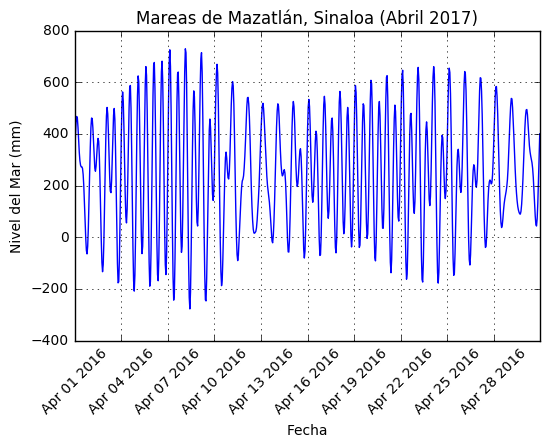
\includegraphics[scale=0.70]{Mazatlang.png}

\vspace{0.5in}

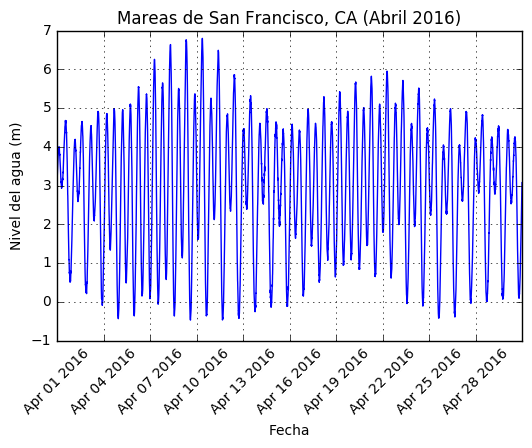
\includegraphics[scale=0.70]{SanFranciscog.png}

\end{center}

\end{document}